%
\section{Communications}
\label{sec:comm}
The communications technologies and the associated tools used for the project development are briefly described next.

\subsection{IEEE 802.11 --- Wi-Fi}%
\label{sec:wifi}
IEEE 802.11, commonly known as Wi-Fi, is part of the IEEE 802 set of \gls{lan} protocols, and specifies the set of \gls{mac2} and
physical layer protocols for implementing \gls{wlan}
communication in a wide sprectrum of frequencies, ranging from 2.4--60 GHz.

\subsubsection{TCP/IP}%
\label{sec:tcpip}
The most commonly used protocols for Internet communications, including Wi-Fi,
are \gls{tcp} and \gls{ip}, usually associated together, being part of the \gls{osi} model
(Fig.~\ref{fig:osi-model}), which characterises and standardises the
communication functions of a telecommunication or computing system, being
agnostic to their underlying internal structure and technology.

A computer protocol is a standardised procedure for the exchange and
transmission of data between devices, as requested for the application processes.
The TCP provides services at the Transport layer, handling the reliable, unduplicated
and sequenced delivery of data~\cite{carne2004professional}, while the UDP provides data transportation
without guaranteed data delivery or acknowledgments. The TCP can be thought of
a reliable version of \gls{udp}, generalizing. The IP part of the TCP/IP suite, providing
services at the Network layer, is used to make origin and destination addresses
available to route data across networks.

These protocols are applied in sequence to the user's data to create a frame
that can be transmitted from the sending application to the receiving
application.
The receiver reverses the procedure to obtain the original user’s data and pass
them to the receiving application~\cite{carne2004professional}.

Another interesting fact, due to the technology agnostic aspect of the OSI
Model, is that IP and the higher-level protocols may be implemented on several
kinds of physical nets.
% OSI model
\begin{figure}[!hbt]
\centering
    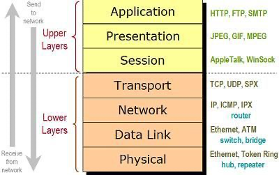
\includegraphics[width=0.5\textwidth]{./img/osi-model.png}
  \caption{\gls{osi} model}%
\label{fig:osi-model}
\end{figure}
%
\subsection{Network programming --- sockets}%
\label{sec:netw-progr-sock}
Computer systems implement multiple processes which require an identifier. As
such, the IP address is not enough to uniquely identify the origin/destination
of data to be transmitted, and the port number is added. This combination of an
IP address and port number is sometimes called a network socket~\cite{wright1995tcp}, allowing
data to be delivered to multiple processes in the same machine --- same IP
address.
It is the socket pair (the 4-tuple consisting of the client IP address, client
port number, server IP address, and server port number) that specifies the two
end points that uniquely identifies each TCP connection in an
internet~\cite{wright1995tcp}. 

In a broader sense, a socket can be described as a method of \gls{ipc} that allows data to be exchanged between applications, either on
the same host (computer) or on different hosts connected by a network~\cite{kerrisk2010linux}, as a
local interface to a system, created by the applications and controlled by the
operating system, allowing an application process to simultaneously send and
receive messages from other processes.

The Socket API was created in UNIX BSD 4.1 in 1981, with widespread
implementation in UNIX BSD 4.2~\cite{kerrisk2010linux}. It implements the Client-Server paradigm and
implement several (standard) functions to access the operating system network
resources, through system calls, in Linux~\cite{kerrisk2010linux}.

There are two generic ways to use sockets: for outgoing connections --- client
socket --- and for incoming connections --- server
socket. Fig.~\ref{fig:sockets-connection} illustrates the required steps to
obtain a connected socket:
\begin{enum-c}
\item When a socket is initially created is mostly unuseful.
\item Binding the server socket associates it to an unique network tuple (address and
  port number), enabling it to be uniquely addressed.
\item When a socket server goes into listening mode, the remote devices can
  initiate the connection procedure, referring to its unique network tuple.
\item When the socket server accepts a connection, it spawns a new socket which
  is connected to the remote device, and the endpoints can effectively
  communicate. The server socket is ready to accept new incomming connections.
\end{enum-c}
% Sockets connection
\begin{figure}[!hbt]
\centering
    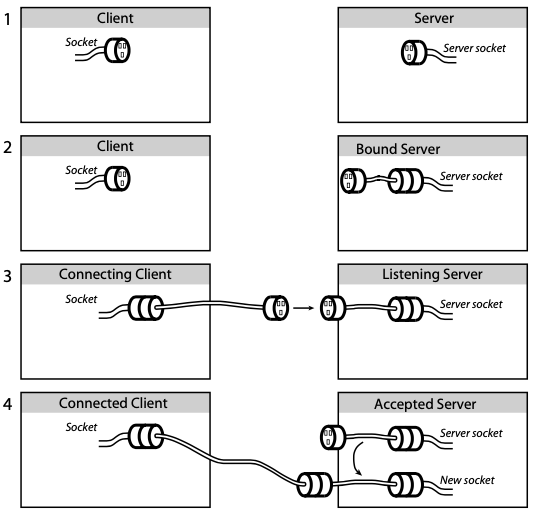
\includegraphics[width=0.6\textwidth]{./img/sockets-connection.png}
  \caption{Steps to obtain a connected socket (withdrawn from~\cite{huang2007bluetooth})}%
\label{fig:sockets-connection}
\end{figure}

\subsection{Client/server model}%
\label{sec:client-serv-model}
The client/server model is the most common form of network architecture used
in data communications today~\cite{hanson2000client}. A client is a system or
application that request the activity of a service provider system or
application, called servers, to accomplish specific tasks.
The client/server concept functionally divides the execution of a unit
of work between activities initiated by the end user (client) and resource responses
(services) to the activity request as a cooperative environment~\cite{hanson2000client}. The client,
typically handling user interactions and data exchange/modification in the user’s
behalf, makes a request for a service, and a server, often requiring some resource
management (synchronization and access to the resource), performs that service,
responding to the client requests with either data or status information~\cite{ibmCliServ}.

An example of a simple client-server model using the Socket \gls{api}, through system
calls, is presented in Fig.~\ref{fig:cli-serv-operation}. The operation of sockets can be explained as
follows~\cite{kerrisk2010linux}:
\begin{itemize}
\item The \texttt{socket()} system call creates a new socket, establishing the
  protocols under which they should communicate. For both client and server to
communicate, each of them must create a socket.
\item  Communication via a stream socket is analogous to a telephone call. One
application must connect its socket to another application’s socket before
communication can take place. Two sockets are connected as follows:
\begin{enumerate}
\item One application, assuming the role of server, calls \texttt{bind()} to
  bind the socket to a well-known address, and then calls \texttt{listen()} to
  notify the kernel it is ready to accept incoming connections.
\item The other application, assuming the role of client, establishes the
  connection by calling \texttt{connect()}, specifying the address of the socket
  to which the connection is to be made.
\item The server then accepts the connection using \texttt{accept()}. If the
  \texttt{accept()} is performed before the client application calls
  \texttt{connect()}, then the \texttt{accept()} blocks.
\end{enumerate}
\item Once a connection has been established, data can be transmitted in both
directions between the applications (analogous to a bidirectional telephone
conversation) until one of them closes the connection using \texttt{close()}.
\item Communication is performed using the conventional \texttt{read()} and
  \texttt{write()} system calls or via a number of socket-specific system calls
  (such as \texttt{send()} and \texttt{recv()}) that provide additional
  functionality. By default, these system calls block if the \gls{io} operation
  can’t be completed immediately. However, nonblocking \gls{io} is also
  possible.
\end{itemize}
% Overview of UNIX system calls
\begin{figure}[!hbt]
\centering
    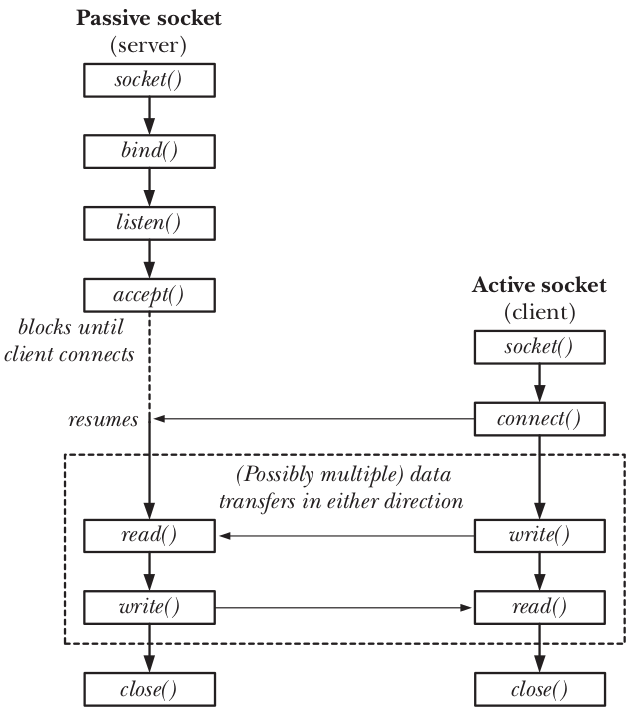
\includegraphics[width=0.62\textwidth]{./img/cli-serv-operation.png}
  \caption{Overview of UNIX system calls with sockets implementing 
a server/client paradigm (withdrawn from~\cite{kerrisk2010linux})}%
\label{fig:cli-serv-operation}
\end{figure}

%%% Local Variables:
%%% mode: latex
%%% TeX-master: "../../../dissertation"
%%% End:
